% !TEX program = xelatex
\documentclass[12pt]{ctexart}
% ------------------------
% 页面
% ------------------------
\usepackage{geometry}
\geometry{margin=2.5cm}

% ------------------------
% 字体
% ------------------------
\usepackage{fontspec}
\setmainfont{Times New Roman}
\setmonofont{Consolas}

% ------------------------
% 基础包
% ------------------------
\usepackage{multirow}
\usepackage{soul}
\usepackage[normalem]{ulem}
\usepackage{lastpage}
\usepackage{xcolor}
\usepackage{hyperref}
\usepackage{graphicx}
\usepackage{booktabs}
\usepackage{enumitem}
\usepackage{caption}
\usepackage{titlesec}
\usepackage{fancyhdr}
\usepackage{tikz}
\usetikzlibrary{arrows.meta, positioning}
% ------------------------
% GitHub 颜色
% ------------------------
\definecolor{gh-bg}{HTML}{FFFFFF}
\definecolor{gh-border}{HTML}{D0D7DE}
\definecolor{gh-codebg}{HTML}{F6F8FA}
\definecolor{gh-link}{HTML}{0969DA}
\definecolor{gh-line}{HTML}{8B949E}

\definecolor{gh-note}{HTML}{0969DA}
\definecolor{gh-warning}{HTML}{9A6700}
\definecolor{gh-tip}{HTML}{1A7F37}

% ------------------------
% 设置页眉与页尾
% ------------------------
\geometry{left=2cm,right=2cm,top=2cm,bottom=2.5cm}
\fancyhf{}
\fancyhead[C]{}
\fancyhead[L]{中国科学院大学·2026年春}
\fancyhead[R]{网络空间安全导论}
\fancyfoot[C]{第 \thepage 页，共 \pageref{LastPage} 页}
\renewcommand{\footrulewidth}{0.4pt}
\renewcommand{\baselinestretch}{1.2}
\pagestyle{fancy}
% ------------------------
% 超链接
% ------------------------
\hypersetup{
	colorlinks=true,
	linkcolor=gh-link,
	urlcolor=gh-link
}

% ------------------------
% 列表间距
% ------------------------
\setlist{
	itemsep=4pt,
	topsep=6pt
}

% ------------------------
% tcolorbox
% ------------------------
\usepackage{tcolorbox}
\tcbuselibrary{minted,skins,breakable}

% ------------------------
% GitHub 引用块
% ------------------------
\newtcolorbox{ghquote}{
	enhanced,
	colback=white,
	colframe=gh-border,
	borderline west={3pt}{0pt}{gh-border},
	arc=2pt,
	left=10pt,
	right=10pt,
	top=6pt,
	bottom=6pt
}

% ------------------------
% GitHub 提示框
% ------------------------
\newtcolorbox{note}{
	enhanced,
	colback=white,
	colframe=gh-note,
	borderline west={4pt}{0pt}{gh-note},
	title=Note
}

\newtcolorbox{warning}{
	enhanced,
	colback=white,
	colframe=gh-warning,
	borderline west={4pt}{0pt}{gh-warning},
	title=Warning
}

\newtcolorbox{tip}{
	enhanced,
	colback=white,
	colframe=gh-tip,
	borderline west={4pt}{0pt}{gh-tip},
	title=Tip
}

% ------------------------
% 代码块
% ------------------------
\usepackage{minted}

\newtcblisting{codeblock}[2][]{
	listing engine=minted,
	minted language=#2,
	minted options={
		linenos,
		breaklines,
		fontsize=\small,
		numbersep=10pt,
		xleftmargin=15pt
	},
	colback=gh-codebg,
	colframe=gh-border,
	arc=6pt,
	boxrule=0.5pt,
	left=6pt,
	right=6pt,
	top=6pt,
	bottom=6pt,
	listing only,
	breakable,
	#1
}


% ------------------------
% 行内代码
% ------------------------
\newtcbox{\inlinecode}{
	on line,
	boxrule=0pt,
	colback=gh-codebg,
	arc=4pt,
	left=3pt,
	right=3pt,
	top=2pt,
	bottom=2pt
}

% ------------------------
% 标题样式
% ------------------------
\titleformat{\section}
{\Large\bfseries}
{\thesection}{0.5em}{}

\titleformat{\subsection}
{\large\bfseries}
{\thesubsection}{0.5em}{}


\renewcommand{\theFancyVerbLine}{\color{gh-line}\small\arabic{FancyVerbLine}}

\newtheorem{application}{应用}
\newtheorem{problem}{问题}
\newtheorem{analogy}{分析}
\newtheorem{experiment}{实验}

% ------------------------
% 修改表头信息
% ------------------------
%改这里可以修改实验报告表头的信息
\newcommand{\name}{陈曦}
\newcommand{\studentNum}{2025K8009970002}
\newcommand{\boxNum}{}
\newcommand{\expNum}{ICS-exp03-01}
\newcommand{\expName}{网络流量分析初步}
\newcommand{\finishdate}{\today}

% ------------------------
% 文档开始
% ------------------------
\begin{document}
	
	\begin{center}
		\LARGE 中国科学院大学·网络空间安全导论实验报告 
	\end{center}
	
	\begin{center}
		\emph{箱子号} \underline{\makebox[4em][c]{\boxNum}}
		\emph{实验序号} \underline{\makebox[8em][c]{\expNum}}
		\emph{实验专题} \underline{\makebox[16em][c]{\expName}}\\
		\emph{小组成员} \underline{\makebox[36em][c]{\name}}\\
		\emph{对应学号} \underline{\makebox[36em][c]{\studentNum}}\\
		\emph{最后修改日期} \underline{\makebox[34em][c]{\finishdate}}
		{\noindent}
		\rule[8pt]{17cm}{0.2em}
	\end{center}
	\begin{abstract}
		本实验以一起企业数据泄露取证为背景，基于 Wireshark 对多份流量文件进行了系统分析。实验首先掌握了抓包过滤、会话追踪及对象导出等基本操作，并通过分析 FTP 与 HTTP 明文流量，直观验证了明文协议导致凭证与文件直接暴露的安全风险。随后，在异常流量中成功识别了 DNS 隧道与 ICMP 隐蔽信道，解码出被窃取的管理员凭证。在综合应用环节，对一份真实攻击流量完成了完整的网络取证：通过协议识别、受害者身份确认、攻击时间线还原与恶意文件提取，揭示了攻击者利用“IP 直连下载站 + 域名 C2 服务器”分离架构实施钓鱼投递、加载器执行、数据外传及横向移动的完整攻击链。结合 IP 归属、域名特征与时间规律，对攻击者进行了多维画像。实验结果表明，明文协议与隐蔽信道的结合构成了严重的数据泄露威胁，企业应全面启用加密通信并部署深度流量监控以抵御此类攻击。
	\end{abstract}
	\section{Wire Shark的初次使用}
	\subsection{工具概述}
	Wireshark工具是网络空间安全中常备的工具，其原理为通过监视物理网卡中的所有流量传输，得到当前网络空间中所有人与网关的信息交换，同时搭配上适当的解析器，最终实现了一个从用户到数据层之间的桥梁。
	\subsection{首次抓包实验}
	开启Wireshark，选择一个网络接口，开始捕获数据包，访问一个特定的网站\href{http://192.3.100.85:5000/}{http://192.3.10}\\\href{http://192.3.100.85:5000/}{0.85:5000/}。观察\hyperref[figure1]{图1}的Wireshark中数据包列表的滚动，其中每一行代表一个数据包。
	
	\vspace{0.5\baselineskip}
	
	\noindent
	\begin{minipage}{\linewidth}
		\label{figure1}
		\begin{center}
			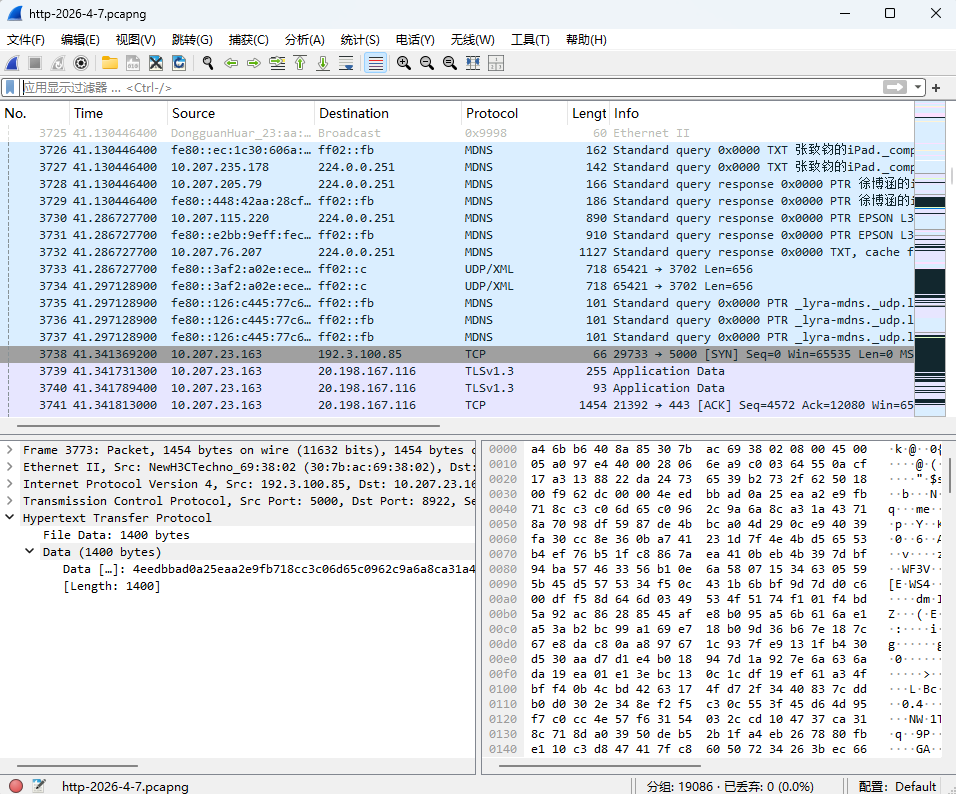
\includegraphics[width=0.3\columnwidth]{pngs/exp1/console.png}
			\captionof{figure}{观察Wireshark中的数据包}
		\end{center}
	\end{minipage}
	为了从成千上万的流量数据中抓取需要的数据，Wireshark提供了许多可选的过滤器与对话数据统计功能，\hyperref[tabular1]{下表}是一些过滤器的示例。在本次测试中我们采用\inlinecode{dns}过滤器进行过滤，得到\hyperref[figure2]{如图2所示}\\
	\begin{minipage}{\linewidth}
			\centering
			\captionof{table}{Wireshark 常用显示过滤器}
			\label{tabular1}
			\begin{tabular}{ll}
				\toprule
				\textbf{过滤器语法} & \textbf{说明} \\
				\midrule
				dns & 仅显示 DNS 协议包 \\
				http & 仅显示 HTTP 协议包 \\
				tls 或 ssl & 仅显示 TLS/SSL 加密流量 \\
				ftp & 仅显示 FTP 控制流量 \\
				icmp & 仅显示 ICMP 协议包（如 ping） \\
				arp & 仅显示 ARP 协议包 \\
				tcp & 仅显示 TCP 协议包 \\
				udp & 仅显示 UDP 协议包 \\
				ip.addr == 192.168.1.1 & 显示与指定 IP 地址相关的所有包 \\
				ip.src == 192.168.1.1 & 仅显示源 IP 为指定地址的包 \\
				ip.dst == 192.168.1.1 & 仅显示目的 IP 为指定地址的包 \\
				tcp.port == 80 & 显示 TCP 端口为 80 的包（HTTP 默认端口） \\
				tcp.srcport == 443 & 仅显示 TCP 源端口为 443 的包 \\
				udp.port == 53 & 显示 UDP 端口为 53 的包（DNS 默认端口） \\
				http.request.method == "GET" & 仅显示 HTTP GET 请求 \\
				http.request.method == "POST" & 仅显示 HTTP POST 请求 \\
				ftp.request.command == "USER" & 仅显示 FTP 用户名传输包 \\
				ftp.request.command == "PASS" & 仅显示 FTP 密码传输包 \\
				dns.qry.name contains "example" & 显示 DNS 查询域名中包含指定字符串的包 \\
				frame contains "password" & 显示数据帧中包含指定关键词的包 \\
				tcp.flags.syn == 1 & 显示 TCP SYN 包（连接请求） \\
				tcp.flags.reset == 1 & 显示 TCP RST 包（连接重置） \\
				\bottomrule
			\end{tabular}
	\end{minipage}\\
	{\color{white} spacespacespace}\hspace*{10em}\\
	\begin{minipage}{\linewidth}
		\label{figure2}
		\begin{center}
			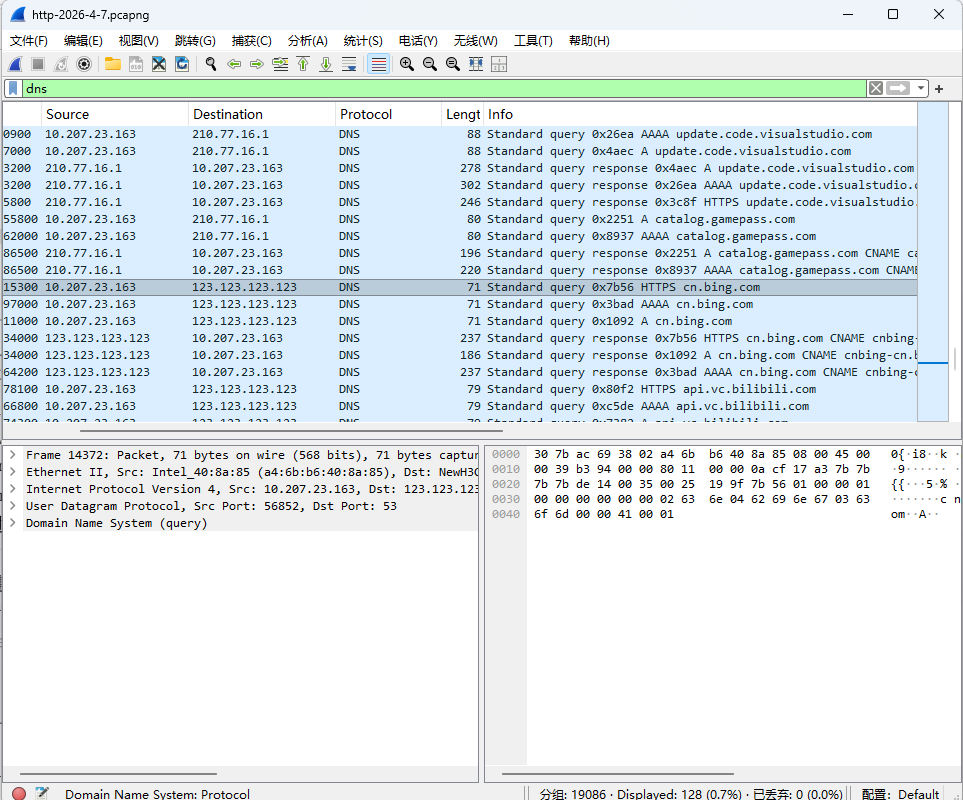
\includegraphics[width=0.3\columnwidth]{pngs/exp1/dns-filter.png}
			\captionof{figure}{使用dns过滤器}
		\end{center}
	\end{minipage}
	观察\inlinecode{Info}列中出现的域名信息和IP地址。 然后使用\inlinecode{右键 → 追踪流 → TCP Stream} 功能打开一段HTTP 对话。观察窗口中红色（请求）和蓝色（响应）的对话内容。
	
	\vspace{0.5\baselineskip}
	
	\noindent
	\begin{minipage}{\linewidth}
		\label{figure3}
		\begin{center}
			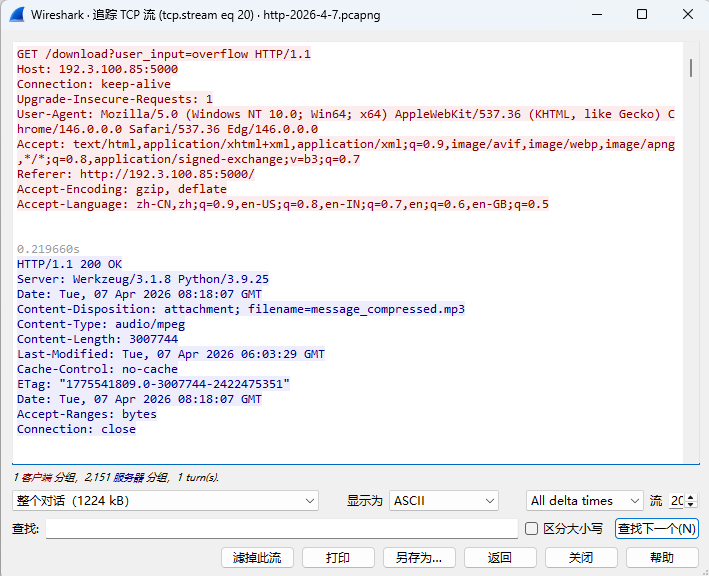
\includegraphics[width=0.3\columnwidth]{pngs/exp1/http-transmision.png}
			\hspace*{2em}
			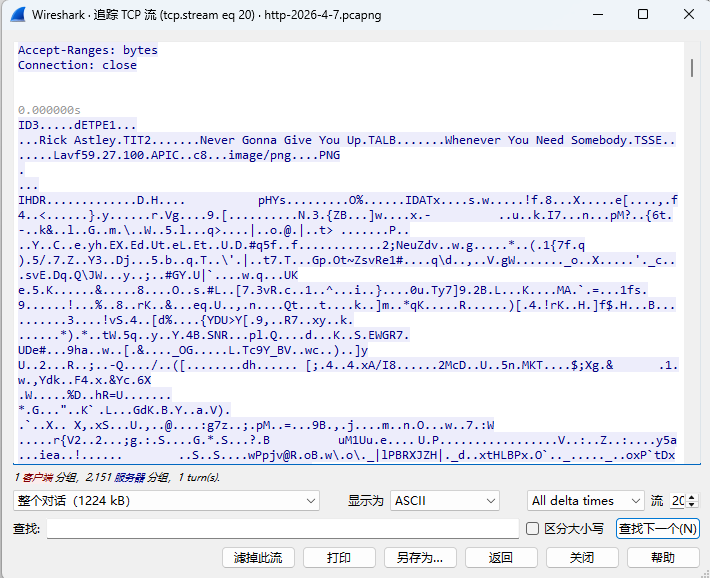
\includegraphics[width=0.3\columnwidth]{pngs/exp1/http-voice-content.png}
			\captionof{figure}{TCP流追踪功能}
		\end{center}
	\end{minipage}
	不难发现客户端与服务器之间采用明文传输(注：\hyperref[figure3]{图三}右半部分的乱码是因为这是音频文件，没有解码)，那么我们尝试使用Wireshark自带的分析工具将客户端与服务器之间的通信内容使用\inlinecode{文件 → 导出对象 → HTTP...}导出一个通过网络传输的文件导出\\
	\begin{minipage}{\linewidth}
		\label{outputfile-http}
		\begin{minipage}{0.4\columnwidth}
			\centering
			\vspace*{1.4\baselineskip}
			
\includegraphics[width=0.3\columnwidth]{pngs/exp1/outputfile.png}
			\captionof{figure}{导出文件图标}
		\end{minipage}
		\hfil
		\begin{minipage}{0.5\columnwidth}
			\centering
			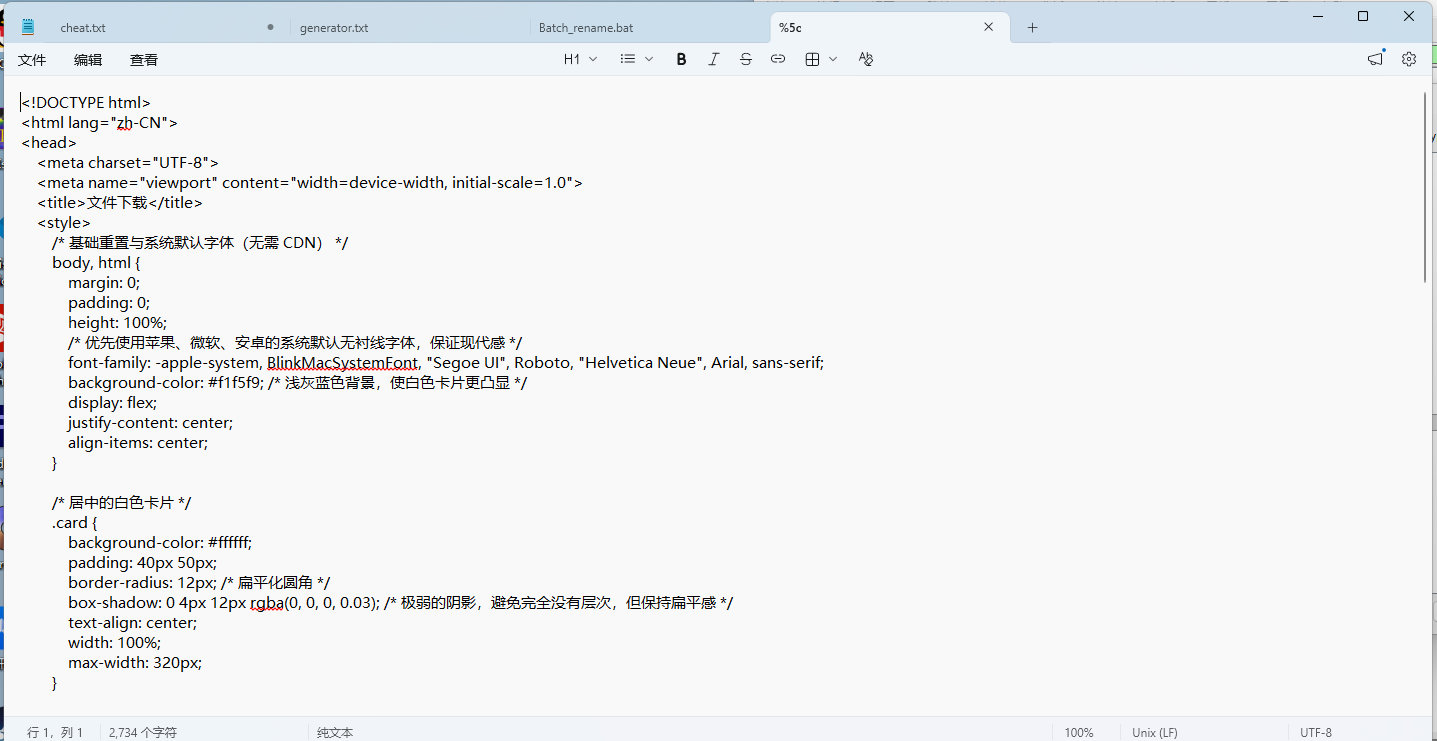
\includegraphics[width=0.6\columnwidth]{pngs/exp1/output-file-content.png}
			\captionof{figure}{导出文件内容}
		\end{minipage}
	\end{minipage}
	于是我们成功实现中间人攻击，成功嗅探到了标靶对象与服务器之间的HTTP通信，也熟悉了Wireshark的基本操作。
	\subsection{DNS解析实验}
	DNS，全称Domain Name System，域名系统，是一个记录域名和IP地址相互映射的一个系统，能够将用户访问互联网时使用的域名地址转换成对应的IP地址，而不用使用者去记住数量众多的IP地址。通过域名得到域名对应的IP地址的过程被称为域名解析。
	
	我们先启动Wireshark，使用\inlinecode{dns}过滤器。然后启动命令提示符，输入
	\begin{codeblock}{bat}
nslookup www.baidu.com
	\end{codeblock}
	
	\vspace*{0.5\baselineskip}
	\noindent
	\begin{minipage}{\linewidth}
		\label{nslookup}
		\centering
		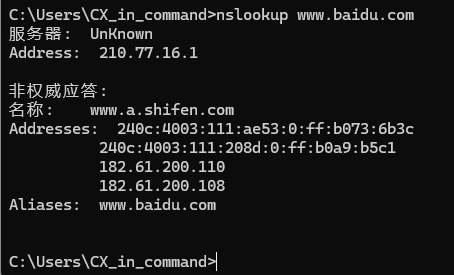
\includegraphics[width=0.25\columnwidth]{pngs/exp2/nslookup.png}
		\captionof{figure}{对百度的域名做DNS解析}
	\end{minipage}
	
	回到Wireshark停止捕获。看到一对数据包：Standard query（查询请求）和Standard query response（查询响应）。\\
	\begin{minipage}{\linewidth}
		\centering
		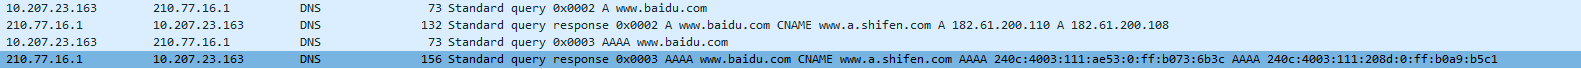
\includegraphics[width=0.6\columnwidth]{pngs/exp2/pack.png}
		\captionof{figure}{Wireshark展示数据包}
	\end{minipage}
	我们打开数据包仔细分析DNS协议所在的应用层数据，我们分别从Queries与Answers两部分分别看到靶机查询的域名与返回的IPV4地址
	
	\vspace*{0.2\baselineskip}
	\begin{minipage}{\linewidth}
		\begin{minipage}{0.4\columnwidth}
			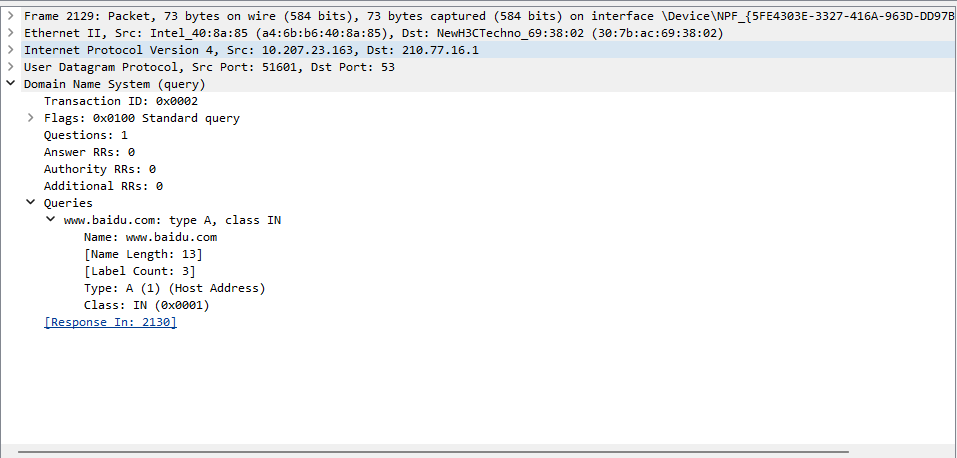
\includegraphics[width=\columnwidth]{pngs/exp2/query.png}
			\captionof{figure}{查询数据包的Queries部分}
		\end{minipage}
		\hfil
		\begin{minipage}{0.4\columnwidth}
			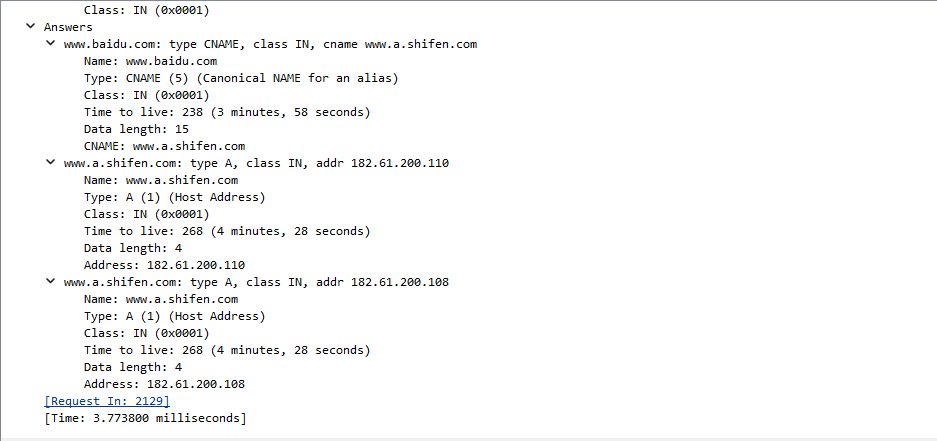
\includegraphics[width=\columnwidth]{pngs/exp2/response.png}
			\captionof{figure}{返回数据包的Answers部分}
		\end{minipage}
	\end{minipage}
	从Wireshark的抓包中不难发现百度为自己的网址同时注册了一个CNAME别名然后引导向了两个IPV4地址(type:A~~的含义就是IPV4，而type:AAAA~~则是IPV6地址)，网站结构如下图\\
	\begin{center}
		\begin{tikzpicture}[
			node distance=1.5cm and 1.5cm,  
			>=Stealth,
			every node/.style={draw, rectangle, align=center}
			]
			% 第一层节点
			\node (sub1) {www.baidu.com};
			\node (sub2) [right=of sub1] {www.a.shifen.com};
			
			% 第二层节点（使用 below left / below right 避免未定义引用）
			\node (sub3) [below left=of sub2] {182.61.200.110};
			\node (sub4) [below right=of sub2] {182.61.200.108};
			
			% 箭头
			\draw[-Stealth] (sub1) -- node[above, sloped, draw=none, fill=white, inner sep=1pt] {映射} (sub2);
			\draw[->] (sub2) -- node[above, sloped, draw=none, fill=white, inner sep=1pt] {DNS解析} (sub3);
			\draw[->] (sub2) -- node[above, sloped, draw=none, fill=white, inner sep=1pt] {DNS解析} (sub4);
		\end{tikzpicture}
		\captionof{figure}{网站结构图}
	\end{center}
	
	同时，在原本的Wireshark展示的数据包的Info部分中，我们发现前面有一组未知编码的数字如0x002、0x003之类。从数据包的详细信息中得知这是其中名字叫做Transaction ID的键值，结合同一组Query\&Response包中共享相同的Transaction ID，可以初步推断得知这个键值用于唯一地标识电脑中每一个DNS响应。
	
	另外，我们也发现DNS服务所采用的也是明文的查询协议，也即所有关键的数据内容不做加密处理，这就存在
	\begin{itemize}
		\item 网页访问信息泄露风险
		\item 被中间人执行DNS劫持风险
	\end{itemize}
	
	同时，由于DNS解析协议属于TLS的前序协议，尽管网站采用某些加密手段加密了网站与客户端之间的通信内容，第三方中间人依然有能力监听到客户端访问的网站对象。
	
	\section{核心实验：谁动了我的密码(\sout{奶酪})}
	\subsection{线索一：明文密码嗅探}
	在抓包得到的pcap包中我们通过使用\inlinecode{ftp}过滤器得到如下的筛选结果\\
	\begin{minipage}{\linewidth}
		\centering
		\label{ftp-filter}
		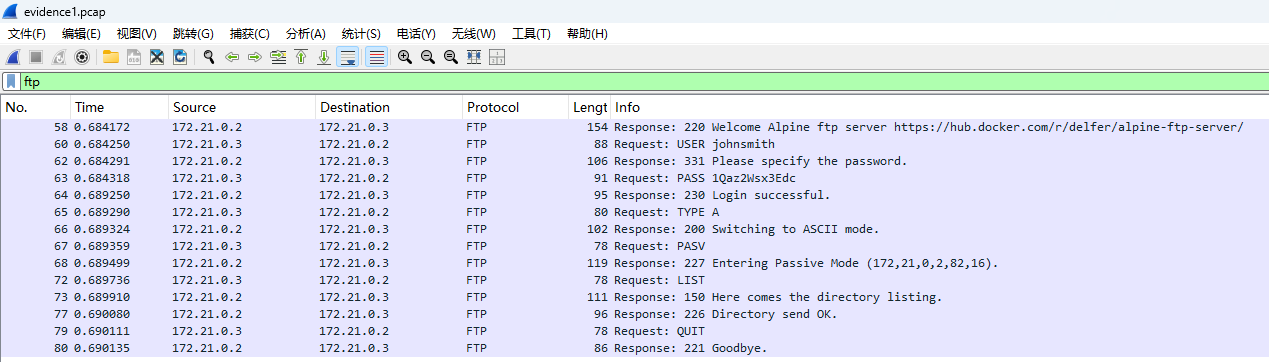
\includegraphics[width=0.4\columnwidth]{pngs/exp3/console.png}
		\captionof{figure}{过滤条件：ftp协议}
	\end{minipage}
	
	不难发现Info列中明文提示词\inlinecode{PASS}、\inlinecode{USER}等字眼，初步推断这位员工账号密码被明文窃取，通过Wireshark的TCP流追踪功能，我们锁定这个可疑账户与公司服务器的通信内容。\\
	\begin{minipage}{\linewidth}
		\centering
		\label{tcp-tracing}
		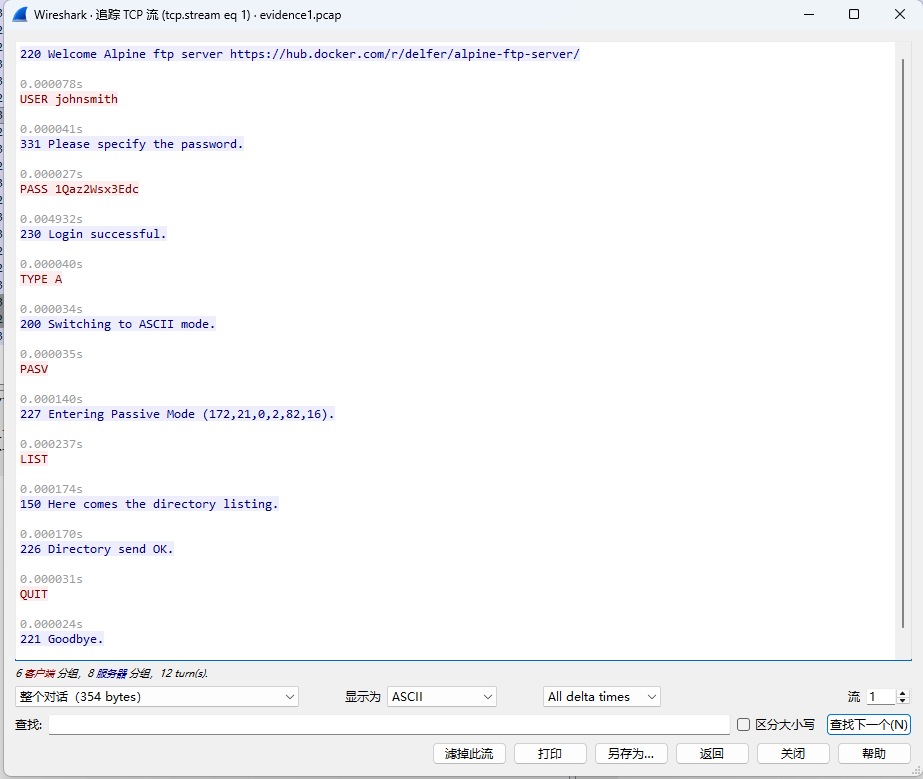
\includegraphics[width=0.4\columnwidth]{pngs/exp3/conversation.png}
		\captionof{figure}{TCP流追踪}
	\end{minipage}
	
	发现这个账户获取了公司敏感文件目录内容，推断攻击者很有可能同步拿到了公司敏感文件目录，推断其具有进一步窃取敏感文件的动机。总结如下：\\
	\begin{minipage}{\linewidth}
		\centering
		\label{summary}
		\begin{tabular}{ll}
			\toprule
			项目& 内容\\
			\midrule 
			用户名& johnsmith\\
			密码 & 1Qaz2Wsx3Edc\\
			登录结果 & 成功，且已经获取敏感内容目录\\
			推测 & 公司敏感文件已经泄露\\
			\bottomrule
		\end{tabular}
		\captionof{table}{网络攻击初步分析总结}
	\end{minipage}
	
	\noindent
	\textbf{问题回应：}
	\begin{enumerate}
		\item 由于FTP是上个世纪计算机刚刚诞生的时期设计的文件传输协议，因此其设计之初就没有考虑到数据需要加密进行传输的需求，因此导致密码被明文暴露在网络环境中，可以被有心人用特殊软件捕捉并识别。这使得攻击者与我(网络安全取证员)几乎没有区别。
		\item 当你在公共WiFi上使用FTP传输文件时，你的用户名、密码以及传输的文件内容，都会以未加密的原始文本（明文）形式在网络上传输。攻击者只需要嗅探就可以获得我在网络中的所有活动，包括文件内容，上网凭证等。这意味着：\textbf{数据泄露，财产损失以及设备被入侵的风险}。
		\item 结合公钥密码学理论，我认为FTP的替代协议应该具有一个TLS/SSL的握手机制，通过交换公钥来实现对对称密钥的加密，然后使用对称密钥加密消息内容，同时在内容中附带上唯一的哈希数字签名。
	\end{enumerate}
	
	\subsection{线索二：文件窃取还原}
	同样，在抓包得到的pcap包中我们使用\inlinecode{http}过滤器得到如下的筛选结果\\
	\begin{minipage}{\linewidth}
		\centering
		\label{open}
		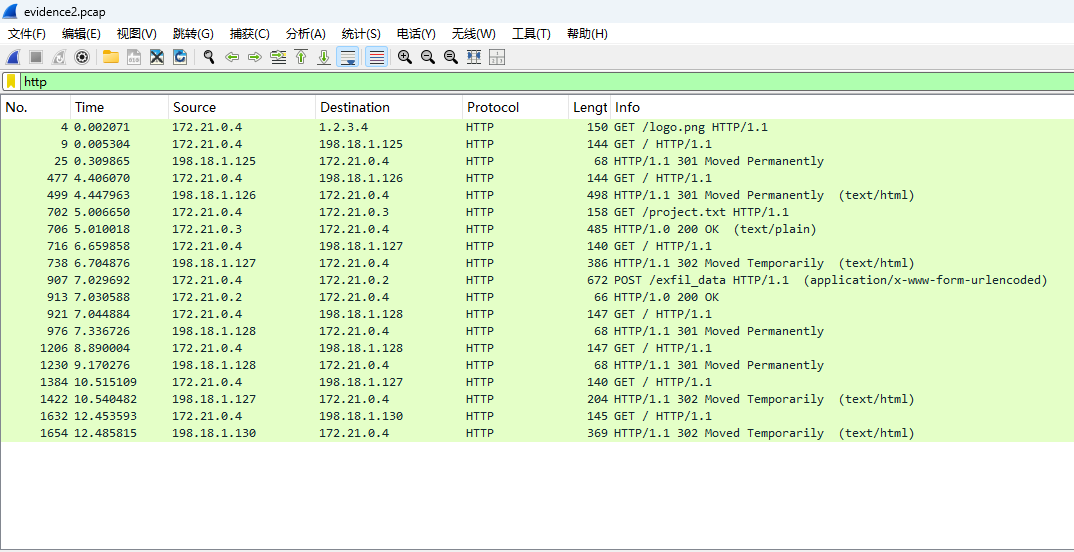
\includegraphics[width=0.4\columnwidth]{pngs/exp4/open.png}
		\captionof{figure}{过滤条件：http协议}
	\end{minipage}
	观察Info列表中的内容，我们发现其中有一条GET与一条POST请求很可疑
	\begin{codeblock}{http}
GET /project.txt HTTP/1.1
Host: internal_srv:8080
	\end{codeblock}
	\begin{codeblock}{http}
POST /exfil_data HTTP/1.1
Host: internal_srv:8080
Content-Type: application/x-www-form-urlencoded
	\end{codeblock}
	我们通过Wireshark尝试将文件导出，发现两份文件内容大致相当，且均为公司的核心机密
	\begin{minipage}{\linewidth}
		\begin{minipage}{0.4\columnwidth}
			\centering
			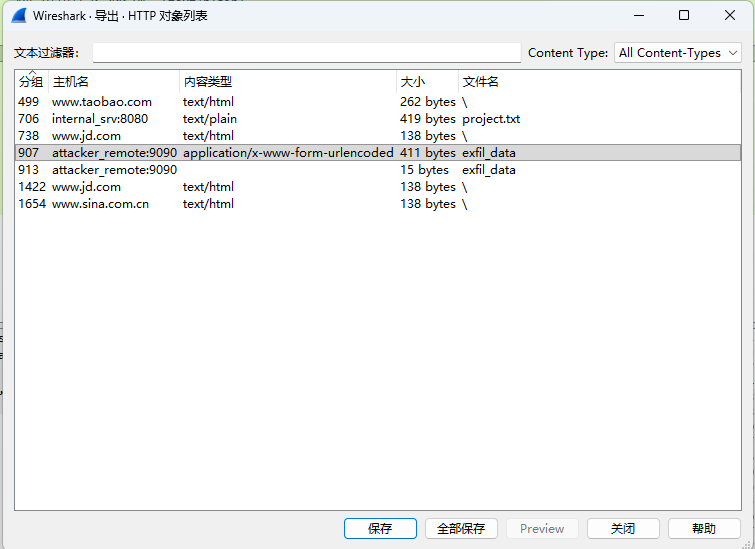
\includegraphics[width=0.6\columnwidth]{pngs/exp4/export.png}
			\captionof{figure}{导出文件}
		\end{minipage}
		\begin{minipage}{0.2\columnwidth}
			\vspace*{1.2\baselineskip}
			\centering
			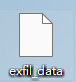
\includegraphics[width=0.6\columnwidth]{pngs/exp4/icon.png}
			\captionof{figure}{文件图标}
		\end{minipage}
		\begin{minipage}{0.4\columnwidth}
			\vspace*{1.8\baselineskip}
			\centering
			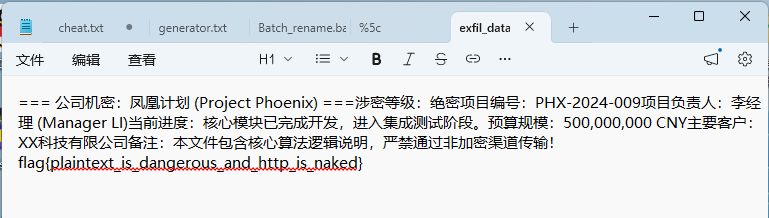
\includegraphics[width=\columnwidth]{pngs/exp4/secret_content.png}
			\captionof{figure}{文件内容}
		\end{minipage}
	\end{minipage}
	
	\noindent
	\textbf{问题回应：}
	\begin{enumerate}
		\item 结合这个部分与上一个部分，我们发现FTP与HTTP的问题共性就是没有采用加密措施导致了内容泄露，严重危害了公司的数据安全。
		\item 我们选择监视本机上观看B站视频，同时启动Edge进行网页浏览作为场景演示。同样监视得到众多数据包，之后选择\inlinecode{统计 → 会话 → Ethernet}选择按照网卡设备MAC地址区分流量\\
		\begin{minipage}{\linewidth}
			\centering
			\label{flow_analyse}
			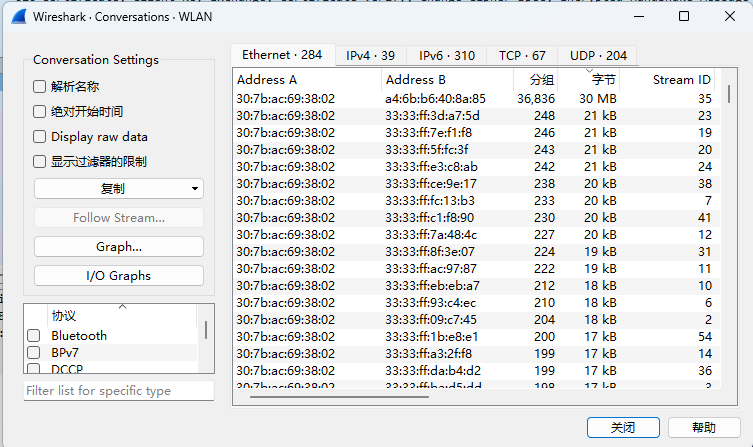
\includegraphics[width=0.4\columnwidth]{pngs/exp4/flow_analyse.png}
			\captionof{figure}{通过MAC地址区分流量}
		\end{minipage}
		不难发现本机由于观看了视频，产生了大量的流量消耗，所以我们右键，选择\inlinecode{查找 → 选中 →}\\\inlinecode{ \(Any \leftrightarrow B\)}对这个目标进行筛选\\
		\begin{minipage}{\linewidth}
			\centering
			\label{filter_AB}
			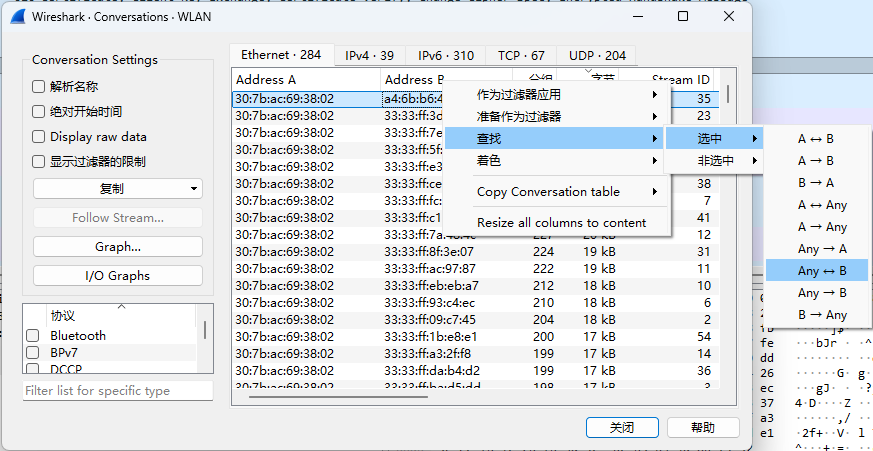
\includegraphics[width=0.4\columnwidth]{pngs/exp4/filter.png}
			\captionof{figure}{使用流量分析功能进行追踪}
		\end{minipage}
		这里选择靶机的一个浏览Edge浏览器的MSN网站(微软版负一屏)作为分析对象，选择对TCP流追踪得到如下结果。发现在没有获取到靶机上的密钥的前提下，即使攻击者在网络空间中进行嗅探，仍然无法得到靶机与服务器之间的通信具体内容。而这就是HTTPS流量的高明之处。(注：TLS握手阶段的SNI字段是明文传输的，因此攻击者可以知道用户访问了哪个域名，但无法知道具体访问了哪个页面或传输了什么数据。)\\
		\begin{minipage}{\linewidth}
			\centering
			\label{https}
			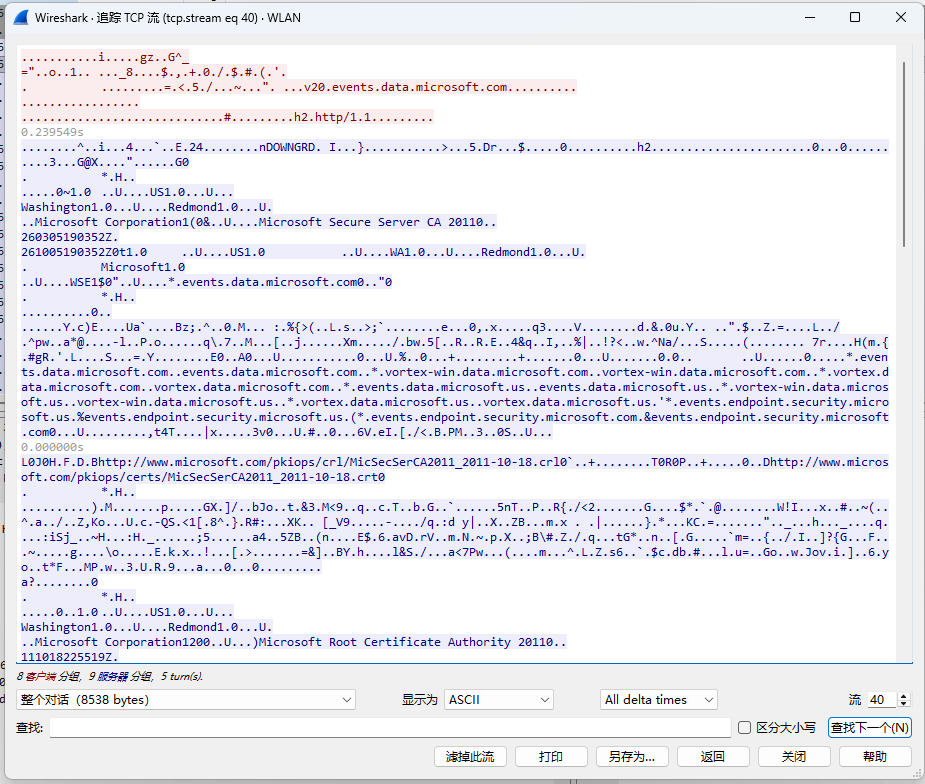
\includegraphics[width=0.4\columnwidth]{pngs/exp4/encrypted.png}
			\captionof{figure}{被加密的HTTPS流量}
		\end{minipage}
		\item HTTPS 本质上就是 在 HTTP 和 TCP 之间插入了一个安全层：TLS（Transport Layer Security，传输层安全协议，其前身是 SSL）。这个安全层提供了加密、数据完整性校验和身份认证三大核心功能，从而解决了 HTTP 明文传输带来的窃听、篡改和冒充风险。
	\end{enumerate}
	\subsection{线索三：隐蔽通信发现}
	\subsubsection{观察DNS查询并使用Base64解码}
	打开evidence3.pcap文件后，在Wireshark主界面上方的显示过滤器输入框中输入“dns”，点击应用按钮或按回车键，仅显示DNS协议相关的数据包。\\
	\begin{minipage}{\linewidth}
		\centering
		\label{dns_serach_cap3}
		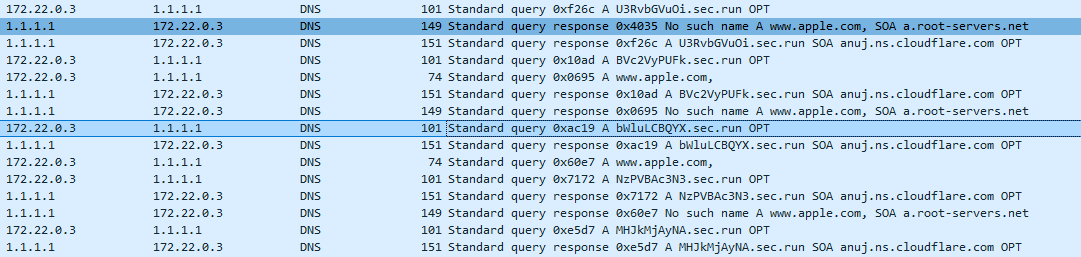
\includegraphics[width=0.4\linewidth]{pngs/exp5/suspecious_dns.png}
		\captionof{figure}{使用dns进行过滤}
	\end{minipage}
	逐一查看DNS查询请求中的“Queries”字段。正常的域名通常由有意义的单词组成，如“baidu.com”\\“mail.qq.com”等，结构规整、可读性强。在浏览过程中，发现大量指向“xxx.sec.run”域名的DNS查询请求。这些查询的子域名部分由随机字符组成，例如：
	\begin{codeblock}{text}
172.22.0.3    1.1.1.1    DNS    101 Standard query 0xac19 A bWluLCBQYX.sec.run OPT
1.1.1.1    172.22.0.3    DNS    151 Standard query response 0xac19 A bwluLCBQYX.sec.run SOA anuj.ns.cloudflare.com OPT
	\end{codeblock}
	收集所有有嫌疑的域名如下
	\begin{codeblock}{text}
U3RvbGVuOi.sec.run
BVc2VyPUFk.sec.run
bWluLCBQYX.sec.run
NzPVBAc3N3.sec.run
MHJkMjAyNA.sec.run
	\end{codeblock}
	拼接之后观察猜测是使用base64编码之后的字符串，使用\href{https://www.toolhelper.cn/EncodeDecode/Base64}{在线base64编解码服务}，将上述字段整理之后解码有\\
	\begin{minipage}{\linewidth}
		\centering
		\label{base64}
		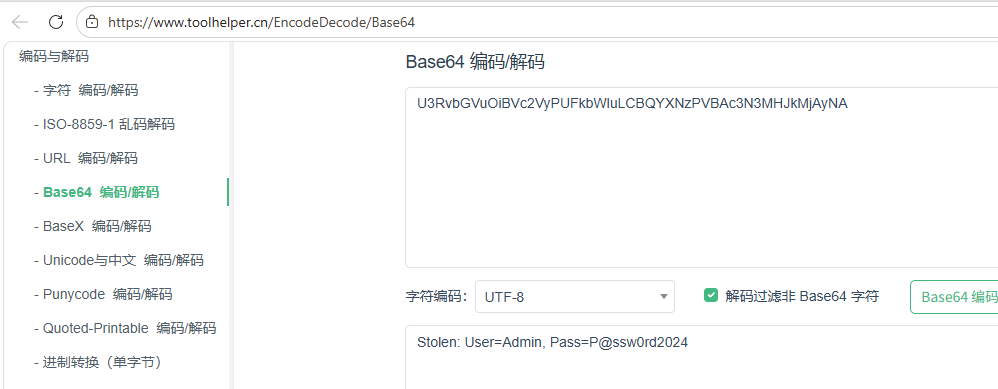
\includegraphics[width=0.4\columnwidth]{pngs/exp5/base64.png}
		\captionof{figure}{使用base64解码}
	\end{minipage}
	得到隐藏信息
	\begin{codeblock}{text}
Stolen: User=Admin, Pass=P@ssw0rd2024
	\end{codeblock}
	\subsubsection{分析ICMP流量}
	首先理解一下什么是ICMP流量：ICMP（Internet Control Message Protocol，互联网控制报文协议）是TCP/IP协议族中的一个子协议，属于网络层协议，用于在IP主机和路由器之间传递控制消息。这些消息主要用于报告网络是否可达、路由是否可用以及数据包传输过程中出现的错误等情况。ICMP本身不传输用户数据，而是作为IP数据包的有效载荷进行封装和传输。
	
	同时注意到ICMP流量有一个可选扩展，可以包含自定义的一些信息。在Wireshark输入icmp，通过对流量的筛查我们发现了两种不同类型的ICMP包。
	
	\vspace*{0.5\baselineskip}
	\begin{minipage}{\linewidth}
		\begin{minipage}{0.5\columnwidth}
			\centering
			\label{normal_ICMP}
			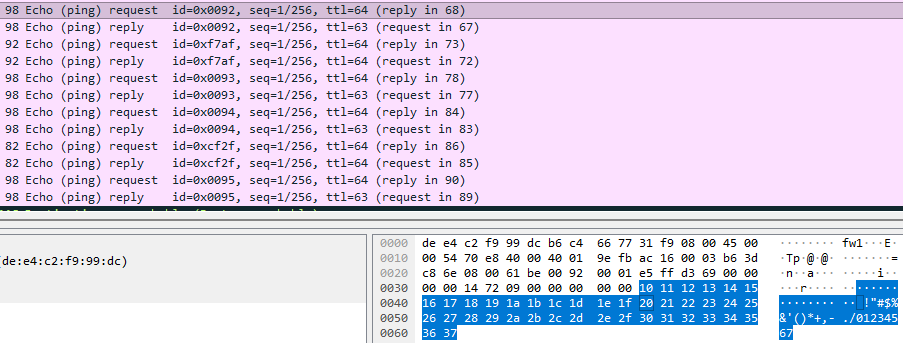
\includegraphics[width=0.8\columnwidth]{pngs/exp5/normal_ICMP.png}
			\captionof{figure}{大多数ICMP包的样式}
		\end{minipage}
		\hfil
		\begin{minipage}{0.5\columnwidth}
			\vspace*{0.8\baselineskip}
			\centering
			\label{abnormal_ICMP}
			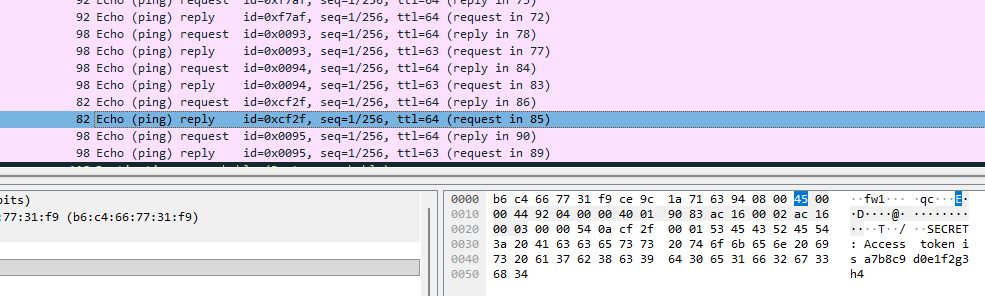
\includegraphics[width=0.8\columnwidth]{pngs/exp5/abnormal_ICMP.png}
			\captionof{figure}{少部分ICMP包的样式}
		\end{minipage}
		
	\end{minipage}
	
	发现大多数的ICMP包仅在最后的可选数据段放了从16-55(以ASCII码编码)这四十个16位数据，但是这个特殊的ICMP包在后面编码了特殊的隐私数据。
	
	\textbf{问题回应}
	\begin{enumerate}
		\item 本次实验在evidence3.pcap文件中发现了两类典型的异常流量：
		
		\textbf{第一类：DNS隧道流量}
		\begin{itemize}
			\item 可疑的父域名：大量DNS查询请求指向“sec.run”这一可疑父域名。正常的企业内网DNS流量中，不太可能出现大量指向同一个陌生域名的查询。
			
			\item 特殊编码的子域名：子域名部分呈现明显的乱码特征。正常域名的子域名由可读的字母和数字组成。
			
			\item 高频重复查询：同一源IP在短时间内向同一父域名发出大量DNS查询，远超正常DNS使用模式。
		\end{itemize}
		\textbf{第二类：ICMP隐蔽通道流量}
		\begin{itemize}
			\item Data字段内容异常：部分ICMP Echo Request数据包的Data字段出现了非标准填充模式的内容。正常的ping数据包使用重复字节模式，而异常包中出现了可读的文本片段或异于常规模板的字符序列。
		\end{itemize}

		\textbf{判断逻辑：}判断以下不正常的流量可以使用下面的几种方法：\textbf{第一、将可疑流量与正常流量模式进行对比。}正常DNS查询的域名具有可读性（如www.baidu.com），而可疑域名呈现高熵随机字符串，两者存在显著差异。正常ICMP包的Data部分为重复填充模式，异常包中出现可读文本。\textbf{第二、可疑流量符合已知攻击模式的特征签名。}DNS隧道攻击的典型特征包括：Base64编码载荷、高频查询同一域名等，本实验观察到的现象与这些特征高度吻合。
		\item 解密数据详见上一部分
		\item 攻击者使用DNS主要有以下几个原因
		
		\hspace*{2em}首先，DNS协议是互联网最基础的协议之一，几乎所有网络环境都会允许DNS流量通过防火墙。防火墙通常默认放行DNS流量，因为如果阻止DNS解析，用户将无法正常访问互联网。攻击者正是利用了这一点——将恶意流量伪装成正常的DNS查询，使其混入海量的合法DNS流量中，难以被传统的安全设备识别和拦截。相比之下，如果攻击者直接向外部服务器发送HTTP请求（使用80或443端口）或原始TCP连接，这些流量很容易被防火墙或出口控制设备识别和拦截，因为企业网络通常会对非HTTP/HTTPS的出站连接进行严格限制。
		
		\hspace*{2em}另一方面，DNS查询遵循递归解析流程：受害主机的DNS查询发送到本地DNS服务器，本地DNS服务器再逐级向上查询直到权威DNS服务器。这意味着攻击者的C2服务器与受害主机之间没有直接的IP连接——所有通信都通过合法的DNS递归解析器中转。这种“中继”结构带来了双重优势：其一，受害主机的真实IP不会直接暴露给C2服务器；其二，安全检测设备更难追踪恶意流量的最终去向，因为看起来只是普通的DNS解析请求。同时也避免了大量流量访问同一个IP地址所可能导致的IP封禁的问题。尽管在DNS隧道方式下，攻击者控制的权威DNS服务器域名虽然也可能被封禁，但攻击者可以快速更换域名或采用临时域名，而受害主机上的恶意程序只需更新DNS解析目标即可恢复通信，防御方难以彻底封堵。
	\end{enumerate}
	\section{回顾复盘}
	
	\subsection*{(1) 还原攻击链}
	
	攻击者首先通过嗅探公司内网流量，截获了员工 John Smith 使用 FTP 协议登录服务器时以明文传输的用户名和密码。随后，攻击者利用该凭据成功登录 FTP 服务器，获取了敏感文件目录列表。接着，攻击者通过 HTTP 协议从内部服务器下载了核心机密文件 \inlinecode{project.txt / exfil\_data }，并将文件内容以 POST 方式外传至外部地址。此外，攻击者还借助 DNS 隧道和 ICMP 隐蔽信道，将窃取到的管理员账号密码（\inlinecode{Admin / P@ssw0rd2024}）分段编码后隐蔽地发送至外部控制端，完成了一次持续性的数据窃取行动。
	
	\subsection*{(2) 根因分析}
	
	整个事件中最根本的安全问题在于：\textbf{关键网络服务采用明文传输协议，且缺乏对网络流量的深度监控能力。} 具体而言，FTP 与 HTTP 协议在设计上未对传输内容进行加密，导致用户名、密码以及文件内容在网络上以明文形式直接暴露。任何能够访问同一网络链路的攻击者，仅需使用 Wireshark 等常规嗅探工具即可轻松窃取这些敏感信息。同时，DNS 与 ICMP 等基础协议的出站流量未被有效管控，使得攻击者能够利用协议的正常功能构建隐蔽信道，绕过传统安全设备的检测。
	
	\subsection*{(3) 防御建议}
	
	\textbf{措施一：全面禁用明文传输协议，强制启用加密替代方案。}
	\begin{itemize}
		\item \textbf{具体内容}：在企业内部全面禁止使用 FTP 和 HTTP 协议进行敏感数据传输。将文件传输服务替换为基于 SSH 的 SFTP 或基于 TLS 的 FTPS；将内部 Web 服务强制升级为 HTTPS。
		\item \textbf{解决的问题}：从根源上杜绝用户名、密码及文件内容在网络传输过程中被明文嗅探的风险。即使攻击者截获了网络数据包，也无法直接读取加密后的通信内容。
	\end{itemize}
	
	\textbf{措施二：部署网络异常行为检测机制，加强对基础协议出站流量的监控。}
	\begin{itemize}
		\item \textbf{具体内容}：在网络边界部署具备深度包检测（DPI）能力的防火墙或入侵检测系统（IDS），并配置针对性的告警规则。例如：监控单台主机在短时间内发起的 DNS 查询频率和域名熵值，对包含高熵随机字符串的 DNS 查询域名进行阻断或告警；对 ICMP 数据包的 Data 字段进行基线建模，对携带非标准填充模式或可读文本的 ICMP 包发出异常警报。
		\item \textbf{解决的问题}：有效识别并阻断攻击者利用 DNS 隧道、ICMP 隐蔽信道等高级技术进行数据外传或远程控制的行为，弥补传统防火墙仅关注 TCP/UDP 端口而忽略协议内容异常的防护盲区。
	\end{itemize}
	\section{问题探究}
		\textbf{(问题一：DNS隐私的攻与防)}传统的DNS查询采用UDP协议的53端口进行明文传输。这意味着，任何能够访问同一网络链路的攻击者，都可以通过Wireshark等工具直接截获并读取DNS请求和响应，从而知道用户访问了哪些网站。这种“明信片”式的通信方式存在严重的隐私泄露风险。为了弥补这一安全缺陷，互联网工程任务组（IETF）制定了两种主流加密DNS协议：DNS over TLS（DoT） 和 DNS over HTTPS（DoH）
		\subsection*{DNS over TLS（DoT）的工作原理}
		DoT由IETF在 RFC 7858 中标准化。其工作原理如下：
		\begin{enumerate}			
			\item 专用端口：DoT使用专用的TCP端口 853 进行通信。
			
			\item TLS加密：客户端与DNS服务器之间建立TLS（Transport Layer Security）加密会话，原始的DNS UDP负载被直接封装在TLS-over-TCP通道中传输。
			
			\item 隐私保护机制：通过TLS加密，DNS查询内容从明文变为密文，网络上的中间人无法窃听用户访问的域名信息。同时，TLS还提供数据完整性校验，防止DNS响应在传输途中被篡改。
			
			\item 特点：DoT“纯粹”地服务于DNS加密，其独立端口853使得企业网络管理员可以较容易地识别、管理和过滤这类流量。
		\end{enumerate}
		\subsection*{DNS over HTTPS（DoH）的工作原理}
		DoH由IETF在 RFC 8484 中标准化。其工作原理如下：
		\begin{enumerate}
			\item 端口复用：DoH不使用独立端口，而是复用标准的HTTPS端口 443。它将DNS查询封装在HTTPS请求中发送。
			
			\item HTTP封装：DNS查询被编码为HTTP GET或POST请求的消息体（MIME类型为application/dns-message），通过TLS加密后，以HTTPS协议发送到DoH解析器。
			
			\item 隐私保护机制：由于DoH流量在端口443上与普通的网页浏览流量完全一致，外部观察者无法从流量特征上区分哪些是DNS查询、哪些是网页访问。这使DoH在抗阻断和隐私隐匿方面表现尤为突出。
			
			\item 特点：DoH对用户隐私的保护更强——攻击者即使截获了数据包，也只能看到TLS加密后的HTTPS流量，无法直接判断哪些包中包含DNS查询内容
		\end{enumerate}
		\subsection{讨论}
		假如所有人都使用了DOH/DOT类似的技术，那么毫无疑问，DNS的安全性得到了保障，使得DNS劫持等网络安全问题发生概率大大降低。但是这也会使得网络安全监控与网络内容监控变得极为复杂。一方面，DoH流量与普通HTTPS流量完全融合，传统的基于53端口的DNS监控手段失效。恶意软件可借助DoH进行通信和数据外传，而安全设备难以检测。另一方面：对于网络安全取证人员而言，加密DNS使得网络流量分析失去了一个重要数据源。在不进行TLS解密的情况下，无法从流量中还原出用户访问的域名信息(注：由于网络环境限制，没有在本机上开启DOH或DOT技术)
		
		\section{综合应用}
		\textbf{(高级网络取证分析)}使用Wireshark打开分析的pcap包，选择\inlinecode{统计 → 协议分级}，得到如下图所示，同时按照网络不同层级整理成表格，并分析有\\
		\begin{minipage}{\linewidth}
			\centering
			\label{protocol-layer}
			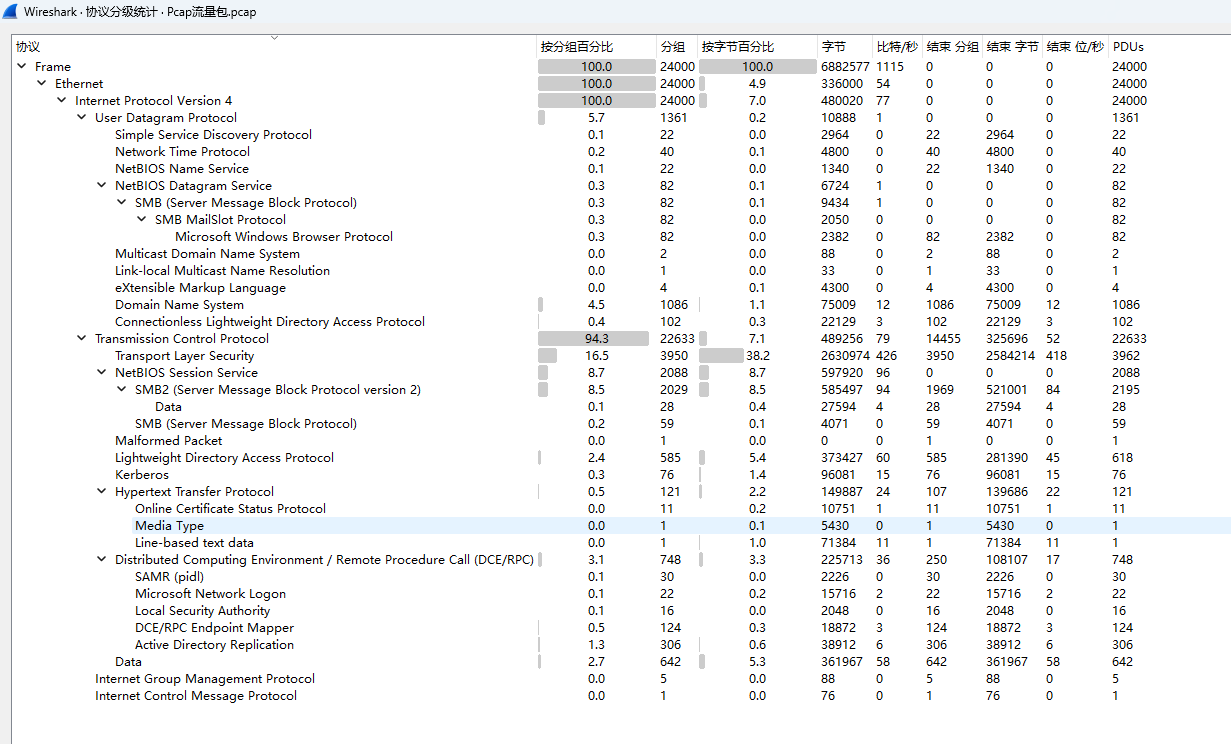
\includegraphics[width=0.6\columnwidth]{pngs/exp6/protocol.png}
			\captionof{figure}{协议识别}
		\end{minipage}
		\textbf{1.链路层}\\
		\begin{minipage}{\linewidth}
			\centering
			\begin{tabular}{lll}
				\toprule
				协议名称	&分组数	&说明\\
				\midrule
				Ethernet&	24000	&底层以太网帧，承载所有上层协议
			\end{tabular}
		\end{minipage}
		
		\vspace*{\baselineskip}
		\noindent
		\textbf{2.网络层}\\
		\begin{minipage}{\linewidth}
			\centering
			\begin{tabular}{lll}
				\toprule
				协议名称&	分组数&	说明\\
				\midrule
				IPv4&	24000&	所有通信均基于 IPv4\\
				ICMP&	1	&仅有 1 个 ICMP 报文（通常用于 ping 或错误报告）\\
				IGMP&	5&	组播组成员管理协议，常用于组播通信\\
				\bottomrule
			\end{tabular}
		\end{minipage}
		
		\vspace*{1\baselineskip}
		\noindent
		\textbf{3.传输层}\\
		\begin{minipage}{\linewidth}
			\centering
			\begin{tabular}{lll}
				\toprule
				协议名称&	分组数&	说明\\
				\midrule
				TCP	&22633&	占比 94.3\%，为主要传输层协议\\
				UDP	&1361&	占比 5.67\%，用于 DNS、NTP、NetBIOS 等服务\\
				\bottomrule
			\end{tabular}
		\end{minipage}
		
		\vspace*{\baselineskip}
		\noindent
		\textbf{4.应用层协议及上层封装}\\
		\begin{minipage}{\linewidth}
			\centering
			\begin{tabular}{llll}
				\toprule
				类别	&协议名称&	分组数&	主要用途\\
				\midrule
				域名解析	&DNS	&1086	&域名查询与响应\\
				&Multicast DNS (mDNS)&	2	&局域网内组播域名解析\\
				&LLMNR	&1	&链路本地多播名称解析（Windows 协议）\\
				文件与打印共享	&SMB&	59 + 82&	SMBv1 版本通信\\
				&SMB2&	2029	&SMBv2 版本通信（占比高，为核心应用）\\
				&NetBIOS Session&	2088&	基于 TCP 的 NetBIOS 会话服务\\
				&NetBIOS Name&	22&	NetBIOS 名称解析\\
			\end{tabular}
		\end{minipage}
		\begin{minipage}{\linewidth}
			\centering
			\begin{tabular}{llll}
				&NetBIOS Datagram&	82&	NetBIOS 数据报服务\\
				&Microsoft Windows Browser&	82&	Windows 计算机浏览服务（网上邻居）\\
				&DCE/RPC&	748&	分布式计算环境远程过程调用（SMB）\\
				目录服务与认证	&LDAP&	585&	轻量目录访问协议\\
				&CLDAP&	102&	无连接 LDAP（UDP）\\
				&Kerberos&	76&	Windows 域认证核心协议\\
				&Active Directory Replication&	306&	AD 复制流量\\
				&SAMR&	30&	安全账户管理器远程协议（账户管理）\\
				&Microsoft Network Logon&	22&	Netlogon 服务\\
				&LSA&	16&	本地安全认证子系统\\
				Web 与加密	&HTTP&	121	&明文 Web 流量\\
				&TLS&	3950&	传输层安全加密\\
				&OCSP&	11&	在线证书状态协议（证书吊销检查）\\
				其他服务&	SSDP&	22&	简单服务发现协议（UPnP 设备发现）\\
				&NTP&	40&	网络时间协议\\
				&XML&	4&	可扩展标记语言（可能为 SOAP 等）\\
				&Media Type&	1&	媒体类型描述\\
				&Line-based text data&	1&	行文本数据（可能是明文协议内容）\\
				异常标记&	Malformed Packet&	1&	Wireshark 解析失败的畸形报文\\
				&Data（应用层无法解析）&	28 + 642&	TCP/UDP 载荷未被正确解析为上层协议\\
				\bottomrule
			\end{tabular}
		\end{minipage}
		\vspace*{0.5\baselineskip}\\
		然后通过分析网络环境中的流量，通过文件导出功能发现网络中存在如下数据交换。注意到其中存在一个以.xyz为顶级域名的域名。这类域名一般属于某些小国家，因为监管宽松而往往成为犯罪分子选择的注册域名，我们之后分析的时候应加以留意\\
		\begin{minipage}{\linewidth}
			\centering
			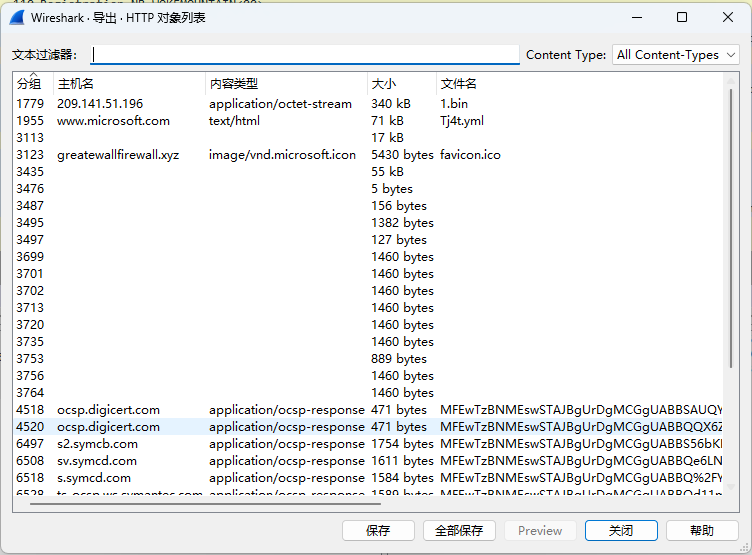
\includegraphics[width=0.5\columnwidth]{pngs/exp6/file_output.png}
			\captionof{figure}{文件导出}
		\end{minipage}
		通过反汇编工具分析得知1.bin是一个加载器，使用了加壳、混淆、环境检测、防调试技术，其中同时存在大量无用代码用于混淆动态调试，因此肯定这是一个木马的一部分。对于导出的文件得到其SHA256指纹为
		\begin{codeblock}{bash}
cx@LAPTOP-K9QOPJ6S:~$ sha256sum 1.bin
236491cfe870f6b374d80e427ef8f8bfbf24f50d4029128b001d95c8c90845cb  1.bin
		\end{codeblock}

		使用wireshark的过滤器进一步追踪1.bin文件的来源IP，\inlinecode{ip.addr == 209.141.51.196 and http}得到
		\begin{codeblock}{text}
No.     Time        Source      Destination     Protocol Length  Info
1308    67.551858   10.1.21.101 209.141.51.196  HTTP     583     GET /files/1.bin HTTP/1.1 
		\end{codeblock}
		所以知道受害者主机的IP地址为10.1.21.101，同时攻击者主机的IP地址为209.141.51.196。使用流量中存在的http请求头信息锁定受害者的MAC地址，浏览器信息及内核信息
		\begin{codeblock}{text}
\\ 数据链路层信息
Source: AcerNetxus_d3:47:8b (00:60:67:d3:47:8b)
.... ..0. .... .... .... .... = LG bit: Globally unique address (factory default)
.... ...0 .... .... .... .... = IG bit: Individual address (unicast)

\\ HTTP请求 header
User-Agent: Mozilla/4.0 (compatible; MSIE 7.0; Windows NT 10.0; WOW64; Trident/7.0; .NET4.0C; .NET4.0E; .NET CLR 2.0.50727; .NET CLR 3.0.30729; .NET CLR 3.5.30729)\r\n
		\end{codeblock}
		所以受害者操作系统是Windows10，Mac地址为00:60:67:d3:47:8b。同时通过UA信息中可知操作系统上安装了多个不同版本的.NET框架，猜测其希望兼容一些老旧的内网程序，但这也可能为攻击者提供机会。进一步扫描受害者主机流量发现SMB/NBNS流量
		\begin{codeblock}{text}
6   0.092205    10.1.21.101 10.1.21.255 NBNS    110 Registration NB DESKTOP-NB72TZA<00>
7   0.092421    10.1.21.101 10.1.21.255 NBNS    110 Registration NB WOKEMOUNTAIN<00>
		\end{codeblock}
		受害者同时注册了主机名DESKTOP-NB72TZA和所在域的NetBIOS域名WOKEMOUNTAIN，表明其已加入wokemountain.com域。这为攻击者后续横向移动提供了条件。综合以上分析，得到受害者指纹
		\begin{codeblock}{text}
IP           : 10.1.21.101
Account Name : DESKTOP-NB72TZA
OS           : Windows 10
Mac          : 00:60:67:d3:47:8b
		\end{codeblock}
		接下来需要深入分析攻击者的远程指令投递机制。受害者主机下载的恶意文件 1.bin 作为一个加载器（Loader），其核心功能是解密并执行内嵌的 Shellcode，随后与真正的命令与控制（C2）服务器建立通信以接收后续指令。为定位该 C2 服务器，使用 Wireshark 过滤器 dns.qry.name contains "greatewallfirewall.xyz" 检查 DNS 流量，发现该域名的 A 记录解析结果为 IP 地址 185.186.244.130。
		
		进一步追踪受害者主机（10.1.21.101）与该 IP 的通信，在绝对时间 125.818640 秒（即 1.bin 文件下载完成约 58 秒后），受害者首先向服务器请求了正常的图标文件（/favicon.ico），随后通过形如 /postfix/[随机编码字符串].yml 的 URI 发起一系列 GET 请求。服务器响应内容为经过 Base64 编码的长字符串，尽管通信信道为明文 HTTP，但实际传输的数据经过了应用层自定义加密处理，其格式与之前下载服务器（209.141.51.196）的明文传输行为截然不同。这些数据被推断为 C2 服务器向加载器下发的加密指令或第二阶段恶意模块。
		
		综合前述所有分析，攻击者的完整攻击路径可归纳为下：

			经深入分析流量时间线，发现受害者主机在下载恶意文件 1.bin（相对时间 67.3 秒）之前，未产生任何关于域名 greatewallfirewall.xyz 的 DNS 查询。受害者直接通过 IP 地址 209.141.51.196 访问了路径 /Lk9tdZ，表明初始攻击链接或恶意宏中硬编码了该 IP。下载服务器返回 302 重定向，最终投递了 DLL 加载器 1.bin。
			
			约 58 秒后（相对时间 125.8 秒），1.bin 执行并主动发起 DNS 查询 greatewallfirewall.xyz，解析至 185.186.244.130，随后与该 IP 建立 HTTP 通信，交换 Base64 编码的加密指令。由此确认，greatewallfirewall.xyz 为第二阶段的 C2 服务器，而之后受害者主机与IP 地址 209.141.51.196保持心跳连接同时回传盗取的敏感资料，攻击者通过C2服务器与回传服务器分离发起攻击。
			\begin{codeblock}{text}
\\ 攻击链条
IP 直连下载站（209.141.51.196）→ 下载 Loader → 执行后解析 C2 域名 → 连接 C2 服务器（185.186.244.130）→ 数据外传与横向移动。
			\end{codeblock}			
		
	\vspace*{\baselineskip}
	\noindent
	\textbf{攻击者画像：}\\
	\hspace*{2em}\textbf{1.通信地址分析：}
	攻击者使用了两台服务器承担下载与命令控制功能，其中209.141.51.196是主要载荷投递服务器和备用C2通道，而185.186.244.130是基于域名的主C2服务器，这里体现了攻击者所做的冗余。：
	\begin{itemize}
		\item 下载服务器 IP：\textbf{209.141.51.196}，经\href{https://whois.ipip.net/}{查询}所属 IP 段为 209.141.32.0/19，归属于 FranTech Solutions，ASN 为 AS53667 (PONYNET)，物理位置位于美国内华达州拉斯维加斯。
		\item C2 服务器 IP：\textbf{185.186.244.130}，经\href{https://whois.ipip.net/}{查询}归属于 AS204957 (LAYER6)，物理位置位于荷兰。该 IP 与域名 \textbf{greatewallfirewall.xyz} 绑定。
	\end{itemize}
	
	\textbf{2.IP服务提供商分析：}
	基于公开信息分析\href{https://www.infosecurity-magazine.com/news/us-web-servers-hosted-10-malware-1/}{[1]}\href{https://cybersecuritynews.com/lockbit-5-0-infrastructure-exposed/}{[2]}\href{https://uk.trustpilot.com/review/frantechusa.com}{[3]}，FranTech Solutions及其关联品牌BuyVM被多家安全研究机构和媒体多次关联到恶意活动：
	\begin{itemize}
		\item 该托管商被描述为 "bulletproof host"（防弹主机），据称其忽略滥用投诉，以言论自由为幌子为非法活动提供便利。
		\item 托管了恶意软件组织LockBit发布的最新一代勒索软件LockBit 5.0的密钥基础设施。
		\item FranTech Solutions被指提供虚假的办公地址，缺乏明确的实体存在，其合法性存疑。
	\end{itemize}
	
	\textbf{3.域名与基础设施分离特征分析：}
	经过对捕获流量的全面分析（见表\ref{domain1}），攻击者采用了“下载服务器裸IP直连 + C2服务器绑定域名”的分离架构：
	\begin{itemize}
		\item \textbf{下载阶段}：受害者直接通过IP地址 \textbf{209.141.51.196} 访问恶意路径 /Lk9tdZ，随后下载载荷 1.bin。全程未涉及任何DNS查询，亦无HTTP Referer。此方式可规避部分基于域名信誉的检测机制，同时便于快速更换下载节点。
		\item \textbf{C2阶段}：载荷执行后，受害主机主动查询域名 \textbf{greatewallfirewall.xyz}，获得A记录 \textbf{185.186.24}\\\textbf{4.130}，随后与该IP建立HTTP会话，通过/postfix/*.yml路径交换Base64编码的加密指令。该域名具有明显嘲讽性质（影射“Great Firewall”），使用廉价顶级域.xyz，符合一次性恶意域名的特征。
	\end{itemize}
	上述分离设计表明攻击者具备一定程度的反侦查意识：下载服务器采用易替换的裸IP，而C2服务器则利用域名实现持久化控制。\\
	\noindent
	\begin{minipage}{\linewidth}
		\centering
		\captionof{table}{域名与IP使用分析}
		\label{domain1}
		\begin{tabular}{ll}
			\toprule
			分析项 & 结论 \\
			\midrule
			下载服务器 HTTP Host 头 & 在 GET /Lk9tdZ 和 GET /files/1.bin 请求中，Host 字段均为209.\\
			& 141.51.196。受害者直接使用 IP 访问。 \\
			C2 通信域名 & 载荷执行后，受害者查询 greatewallfirewall.xyz 并解析至185.1\\
			& 86.244.130。后续 C2 请求中 Host 头为该域名。 \\
			TLS SNI 字段 & 在后续 C2 通信中（若存在 TLS 握手），Server Name Indication\\
			& 字段应包含 greatewallfirewall.xyz（本流量中 C2 信道为明文H-\\
			& TTP，故无 SNI）。 \\
			下载阶段 DNS 查询 & 受害者发起对 209.141.51.196 的连接前，\textbf{未捕获到}任何相关D-\\
			& NS 查询。 \\
			流量中出现的其他域名 & 除内网域 wokemountain.com 及正常流量（bing.com、microsoft\\
			&.com）外，仅发现恶意域名 greatewallfirewall.xyz。 \\
			\bottomrule
		\end{tabular}
	\end{minipage}
	
	\vspace*{\baselineskip}
	\textbf{4.时间规律分析：}\\
	\begin{minipage}{\linewidth}
		\centering
		\captionof{table}{时间规律分析}
		\begin{tabular}{lll}
			\toprule
			时间字段 & UTC时间 & 说明 \\
			\midrule
			Date（下载服务器响应） & 2021-01-20 23:40:38 & 攻击发生时间 \\
			Last-Modified（载荷文件） & 2021-01-20 16:37:34 & Payload生成/上传时间 \\
			Cookie Expires（跟踪Cookie） & 2021-02-20 23:40:38 & 30天有效期 \\
			JWT time & 1611186038（=23:40:38） & 与请求时间一致 \\
			C2 首次通信 & 2021-01-20 23:41:43（约） & 载荷下载后约58秒 \\
			\bottomrule
		\end{tabular}
	\end{minipage}
	\begin{itemize}
		\item Payload生成时间与攻击发生时间相差约7小时，说明攻击者在攻击当天准备了payload，而非使用陈旧文件。
		\item Cookie有效期为30天，符合僵尸网络长期管理的常见周期。
		\item 攻击发生于UTC 23:40（美国东部时间18:40，欧洲深夜），无明显节假日特征，但C2通信紧接其后，显示攻击链高度自动化。
	\end{itemize}

\end{document}
